\section{DTW: Dynamic Time Warping}
Il \textbf{Dynamic Time Warping} (DTW)\cite{dtw}è un algoritmo per misurare la similarità tra due TS, calcolandone il match ottimale.\\
\\
A differenza delle classiche funzioni di distanza, come quella Euclidea o la Manhattan, essa effettua un confronto di tipo \textbf{elastico} (non-lineare) tra i punti delle due TS a confronto: Esse non sono confrontate 1-a-1, matchando l'$i$-esimo punto della TS A con l'$i$-esimo punto della TS B, bensì 1-a-n, matchando un punto della TS A con uno o più punti della TS B.\\
Il confronto tra due punti matchati avviene sempre con una metrica classica, come quella Euclidea. Tutte le singole distanze tra i punti sono conservate in una \textbf{matrice di distanza}.\\
\\
Siano A e B due TS a confronto, vengono imposti i seguenti vincoli nel clacolo del DTW:
\begin{itemize}
	\item Un punto di una TS può essere matchato con uno o più punti dell'altra TS;
	\item Il match tra due punti può avviene se e solo se le due TS hanno la stessa monotonia nei rispettivi punti;
	\item Il primo punto della TS A è matchato con il primo della TS B;
	\item L'ultimo punto della TS A è matchato con l'ultimo della TS B; 
\end{itemize}
\begin{figure}[H]
	\centering
	\begin{subfigure}{.5\textwidth}
		\centering
		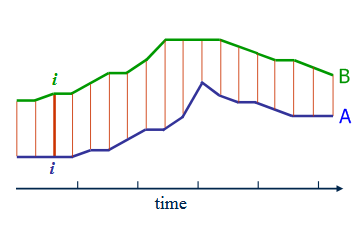
\includegraphics[width=.9\linewidth]{euclidean.png}
		\caption{Distanza Euclidea (lineare)}
		\label{fig:distance_euclidean}
	\end{subfigure}%
	\begin{subfigure}{.5\textwidth}
		\centering
		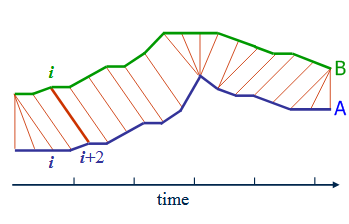
\includegraphics[width=.9\linewidth]{dtw.png}
		\caption{DTW (elastica)}
		\label{fig:distance_dtw}
	\end{subfigure}
	\caption{Confronto tra distanza Euclidea e DTW}
	\label{fig:distance}
\end{figure}
In altre parole, il DTW cerca di "allineare" al meglio le due TS, facendo in modo che entrambe proseguano con lo stesso andamento.\\
\\
La similarità del DTW produce buoni risultati per le TS che rappresentano uno stesso evento ma che sono di lunghezza differente, ad esempio quando entra in gioco uno sfasamento temporale.\\
Un individuo che pronuncia una stessa frase con lo stesso tono ma con velocità differente produrrebbe due TS molto differenti. Se esse venissero confrontate linearmente, non si potrebbe riconoscere che, difatti, l'individuo che ha prodotto tali frequenze è lo stesso. Con un confronto tramite DTW ciò viene ovviato.\\
\\
L'algoritmo compie una ricerca nella matrice di distanza, di spazio $O(mn)$, dove $m$ ed $n$ sono le lunghezze delle due TS confrontate.
Dunque, al caso pessimo e con TS molto grandi (es. centinaia di punti), il calcolo del DTW richiede un tempo impraticabile. In letteratura, perciò, sono state definite alcune implementazioni veloci, come \textit{PrunedDTW}, \textit{SparseDTW} e \textit{FastDTW}, che tentano di accelerarne il calcolo. Ciò nonostante, la tecnica resta complessa in termini di tempo e di spazio, sopratutto in caso di dataset ad alta dimensionalità.\\

\section{Confronto con k-Means di TSLearn}
Il clustering mediante l'impiego di DWT è stato realizzato sfruttando la libreria TSLearn.
Essa, infatti, come evidenziato dal nome stesso, consiste in una specializzazione del Machine Learning focalizzato sulle Time Series.
La libreria non solo offre metodi per il calcolo delle metriche proprie delle TS (\textit{DTW},\textit{Soft-DTW}, ecc.), ma anche veri e propri algoritmi di Machine Learning in una variante modificata \textit{ad hoc} per le TS, sia di tipo supervised che unsupervised (es. \textit{SVM}, \textit{TimeSeriesKMeans}).\\
\\
Proprio uno di questi algoritmi, \textit{TimeSeriesKMeans}, è stato impiegato per il nostro esperimento.
Esso consiste in una versione modificata del noto algoritmo di clustering, abile nel calcolo dei cluster usando non solo la metrica euclidea, ma anche il DTW e il Soft-DTW.\\
\\
Di seguito sono riportati i risultati del clustering dei dataset in esame, con però alcune premesse:
\begin{itemize}
	\item Il Silhouette Coefficient per tutti i dataset, data l'impraticabilità di calcolo su dataset di grandi dimenioni;
	\item Non viene riportata la Relative Purity perché introdotta successivamente al calcolo di questi risultati, e una sua introduzione avrebbe richiesto un computo troppo oneroso;
	\item Per avere un riscontro diretto con le labels presente nei dataset, il numero di cluster calcolati corrisponde al numero di classi presenti nel dataset;
\end{itemize}

\begin{center}
	\pgfplotstabletypeset[
	col sep=comma,
	string type,
	every head row/.style={
		before row={\hline
			\multicolumn{3}{c|}{\textbf{}} &
			\multicolumn{2}{c|}{Internal} & \multicolumn{3}{c}{External} \\
		},
		after row=\hline
	},
	every last row/.style={after row=\hline},
	]{metrics/dtw/All_dtw.csv}
	\begin{table}[H]
		\centering
		\caption{k-Means con DTW sui dataset in esame con relative misure.}
	\end{table}
\end{center}

Da questi risultati è possibile fare una serie di osservazioni:
\begin{enumerate}
	\item In \textit{ECG5000}, \textbf{l'autoencoder e TSLearn con 5-Means hanno tutti gli score molto simili}.\\
	L'autoencoder è riuscito ad estrarre bene le caratteristiche degli elettrocardiogrammi, come intuito dall'analisi precedente;

	\item In \textit{ECG200}, \textbf{l'autoencoder con 2-Means ha tutti gli score leggermente migliori rispetto a TSLearn}.\\
	Le motivazioni sono le stesse di ECG5000;

	\item In \textit{ChlorineConcentration}, \textbf{l'autoencoder e TSLearn su 3-Means hanno tutti gli score molto simili}, se non per una leggera differenza per FMI.\\
	L'autoencoder è riuscito ad estrarre bene le caratteristiche di questo tipo di TS, cosa non intuita dall'analisi precedente;

	\item In \textit{FordA}, \textbf{l'autoencoder con 2-Means ha tutti gli score ben peggiori rispetto a TSLearn}, ad eccezione del FMI, dove in entrambi i casi è comunque non ottimale.\\ L'autoencoder non è riuscito ad estrarre bene le caratteristiche di queste TS "rumorose", come intuito dall'analisi precedente;

	\item In \textit{FordB}, \textbf{l'autoencoder con 2-Means ha gli score interni ben peggiori di quelli di TSLearn}, mentre quelli esterni sono simili.\\
	Similmente a FordA, l'autoencoder non è riuscito ad estrarre bene le caratteristiche di queste TS, come intuito dall'analisi precedente;

	\item In \textit{PhalangesOutlineCorrect}, \textbf{l'autoencoder con 2-Means ha qualche score leggermente peggiore rispetto a TSLearn}.\\
	L'autoencoder è riuscito ad estrarre abbastanza bene le caratteristiche di questo tipo di TS, magari c'è bisogno di alcune modifiche agli iperparametri per poter migliorarne la qualità;

	\item In \textit{RefrigerationDevices}, \textbf{l'autoencoder con 3-Means ha tutti gli score ben peggiori rispetto a TSLearn}, ad eccezione del FMI, dove in entrambi i casi è comunque non ottimale.\\
	Quasi identicamente a FordA, l'autoencoder non è riuscito ad estrarre bene le caratteristiche di queste TS "rumorose", come intuito dall'analisi precedente;

	\item In \textit{TwoLeadECG}, \textbf{l'autoencoder e TSLearn con 2-Means hanno tutti gli score molto simili}, ad eccezione del DB dove l'autoencodere è migliore.\\
	Questa analisi non è pienamente affidabile perché il test set fornito è troppo piccolo, quindi gli score sono soggetti a molte variazioni in caso di riesecuzioni.

	\item In \textit{TwoPatterns}, \textbf{l'autoencoder con 4-Means ha tutti gli score ben peggiori rispetto a TSLearn}, ad eccezione del DB, dove resta comunque non ottimale.\\
	Similmente a FordA, l'autoencoder non è riuscito ad estrarre bene le caratteristiche di queste TS "rumorose", come intuito dall'analisi precedente;
\end{enumerate}

\section{Confronto con altre tecniche di feature extraction and selection}
Sono stati reperiti alcuni risultati di clustering sui dataset in esame attuando però altre tecniche di feature extraction and selection. Il clustering è stato fatto con k-Means con k pari al numero di classi del dataset e su un numero differente di feature estratte in modo diverso:
\begin{itemize}
	\item \textbf{Tutte le feature estratte} da \textit{TSFresh};
	\item \textbf{Feature rilevanti} selezionate da \textit{TSFresh};
	\item Feature rilevanti selezionate dall'algoritmo \textbf{NDFS};
	\item Feature rilevanti selezionate dall'algoritmo \textbf{Lap Score}.
\end{itemize}
I seguenti risultati riportano solo gli score silhouette, Davies-Bouldin e purity, quindi verranno usati solamente questi per il confronto.

\subsubsection{ECG5000}
\begin{figure}[H]
	\centering
	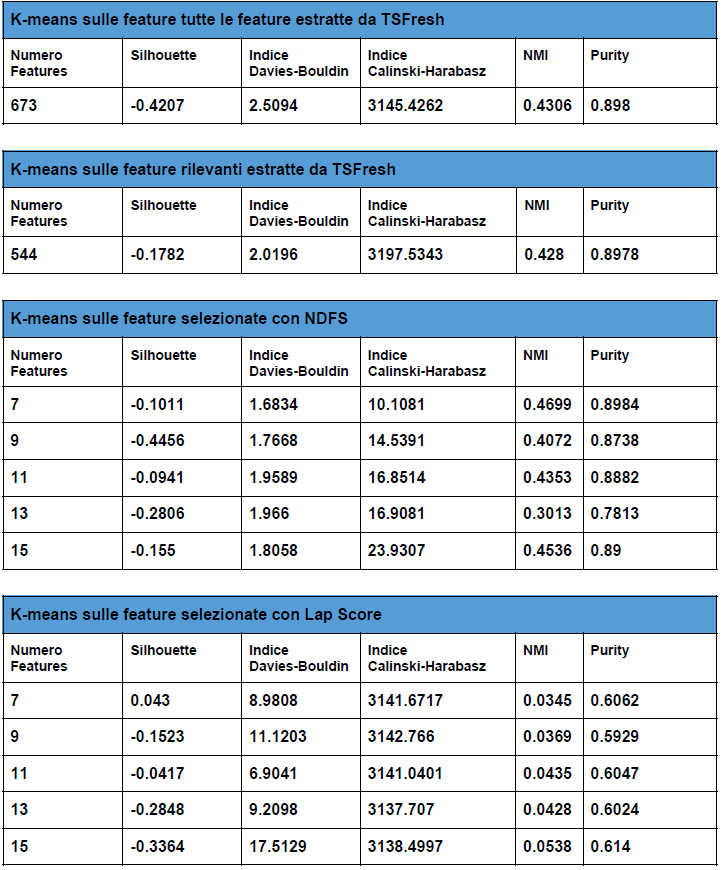
\includegraphics[width=0.9\linewidth]{av/ecg5000_av.png}
	\caption{ECG5000 con tecniche di feature extraction and selection.\\
	\\
	\textbf{L'autoencoder ha migliore silhouette rispetto a tutti gli algoritmi}. DB e Purity sono simili per autoencoder, TSFresh ed NDFS. Lap Score ha gli score peggiori.}
	\label{fig:ecg5000_av}
\end{figure}

\subsubsection{ECG200}
\begin{figure}[H]
	\centering
	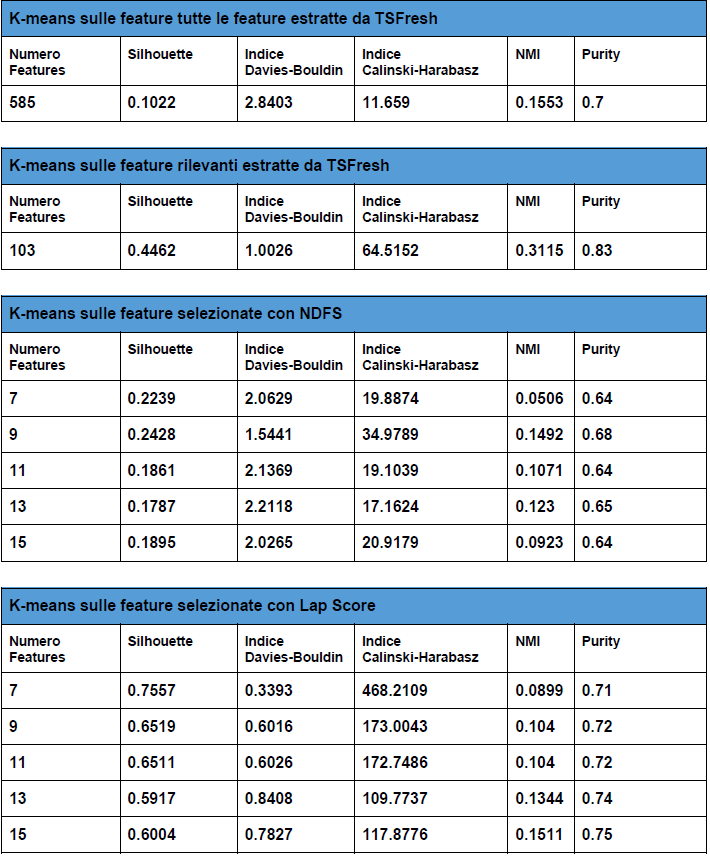
\includegraphics[width=0.9\linewidth]{av/ecg200_av.png}
	\caption{ECG200 con tecniche di feature extraction and selection.\\
	\\
	\textbf{L'autoencoder ha migliore DB rispetto a tutti gli algoritmi, e silhouette migliore rispetto a TSFresh e NDFS, ma peggiore rispetto a Lap Score}. La purity è simile per autoencoder, TSFresh e Lap Score.}
	\label{fig:ecg200_av}
\end{figure}

\subsubsection{ChlorineConcentration}
\begin{figure}[H]
	\centering
	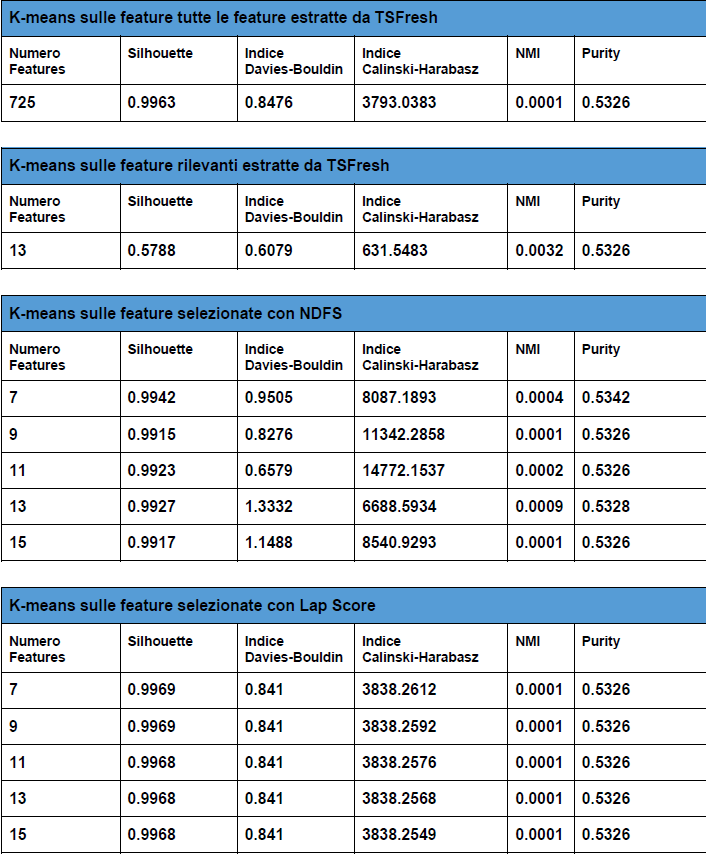
\includegraphics[width=0.9\linewidth]{av/chlorine_av.png}
	\caption{ChlorineConcentration con tecniche di feature extraction and selection.\\
	\\
	\textbf{L'autoencoder ha purity simile a tutti e quattro gli algoritmi}, DB peggiore solo rispetto a TSFresh per feature rilevanti, e silhouette peggiore in tutti i casi, specialmente rispetto ad NDFS e Lap Score, nei quali è quasi massima.}
	\label{fig:chlorine_av}
\end{figure}

\subsubsection{FordA}
\begin{figure}[H]
	\centering
	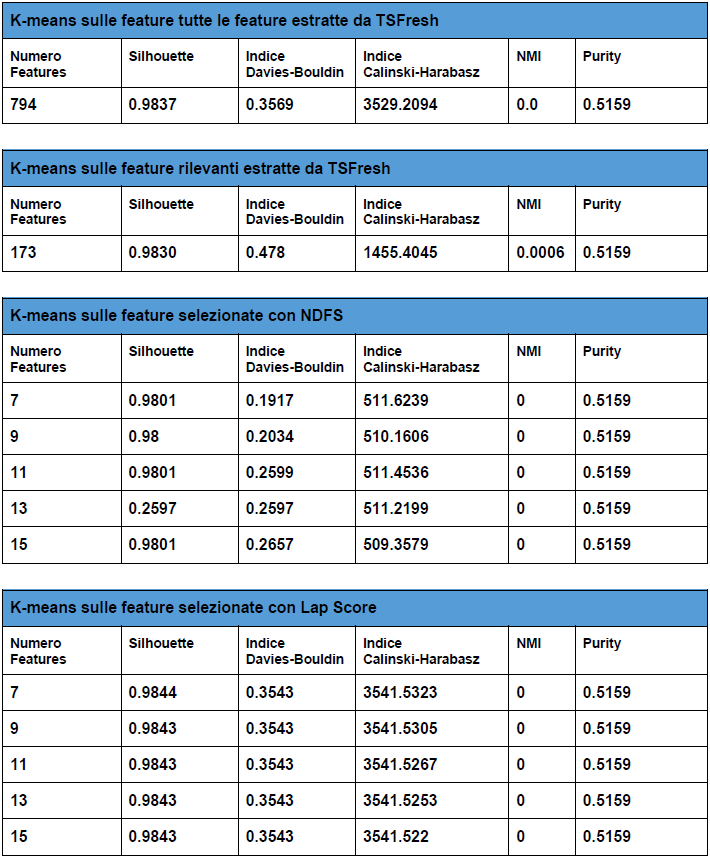
\includegraphics[width=0.9\linewidth]{av/forda_av.png}
	\caption{FordA con tecniche di feature extraction and selection.\\
	\\
	\textbf{L'autoencoder ha silhouette e DB di gran lunga peggiori rispetto a quattro gli algoritmi}, mentre la purity è simile in tutti i casi. DB è quasi ottimale con NDFS.}
	\label{fig:forda_av}
\end{figure}

\subsubsection{FordB}
\begin{figure}[H]
	\centering
	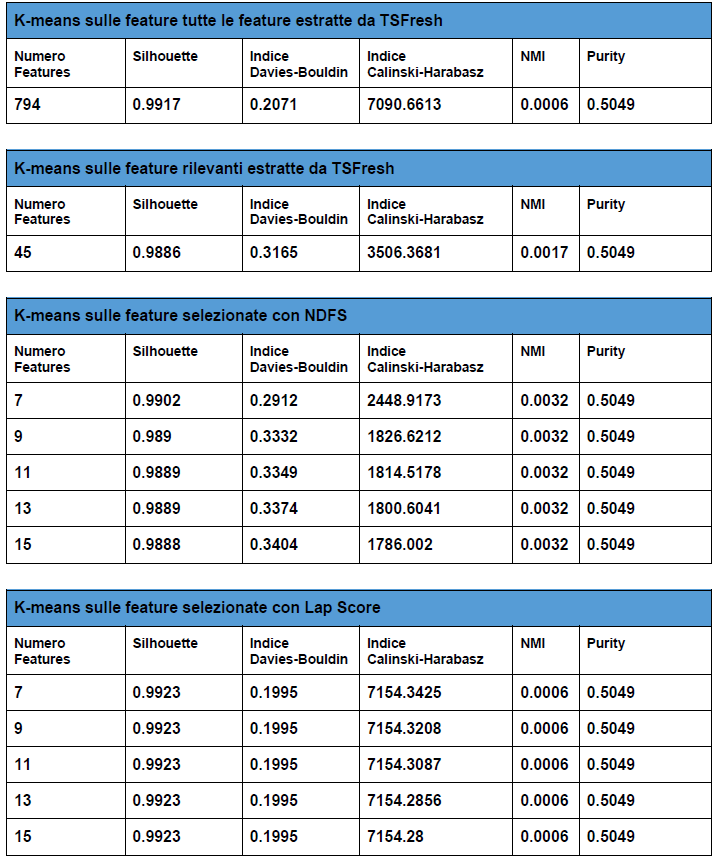
\includegraphics[width=0.9\linewidth]{av/fordb_av.png}
	\caption{FordB con tecniche di feature extraction and selection.\\
	\\
	\textbf{L'autoencoder ha silhouette e DB di gran lunga peggiori rispetto a quattro gli algoritmi}, mentre la purity è simile in tutti i casi. DB è quasi ottimale con Lap Score. E' una situazione simile a quella di FordA.}
	\label{fig:fordb_av}
\end{figure}

\subsubsection{PhalangesOutlineCorrect}
\begin{figure}[H]
	\centering
	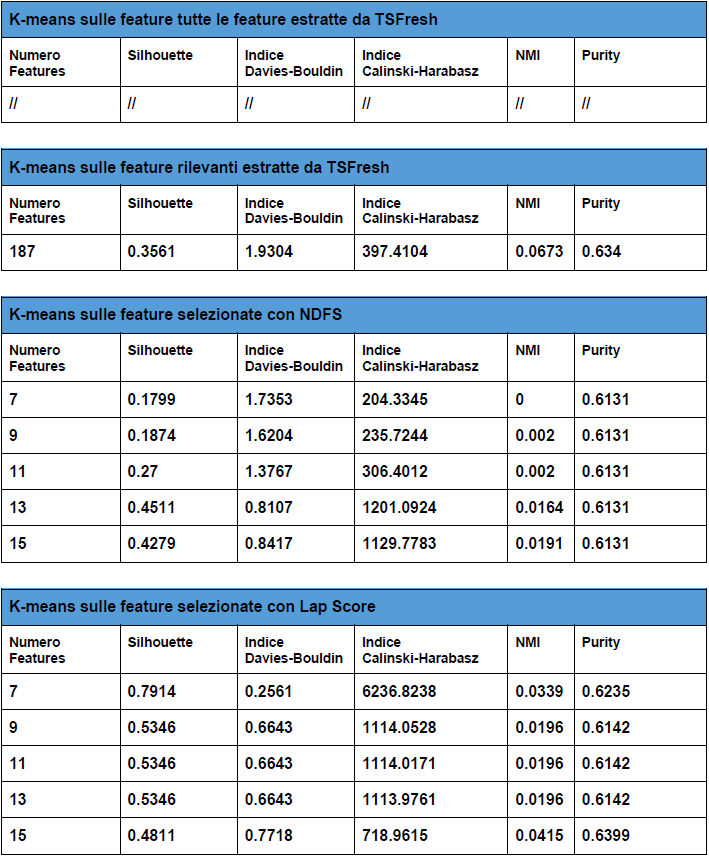
\includegraphics[width=0.9\linewidth]{av/phalanges_av.png}
	\caption{PhalangesOutlineCorrect con tecniche di feature extraction and selection.\\
	\\
	\textbf{L'autoencoder ha purity simile a tutti e quattro gli algoritmi}, mentre ha silhouette e DB variabili: migliori rispetto a TSFresh e una parte di NDFS, peggiori rispetto a Lap Score e un'altra parte di NDFS.}
	\label{fig:phalanges_av}
\end{figure}

\subsubsection{RefrigerationDevices}
\begin{figure}[H]
	\centering
	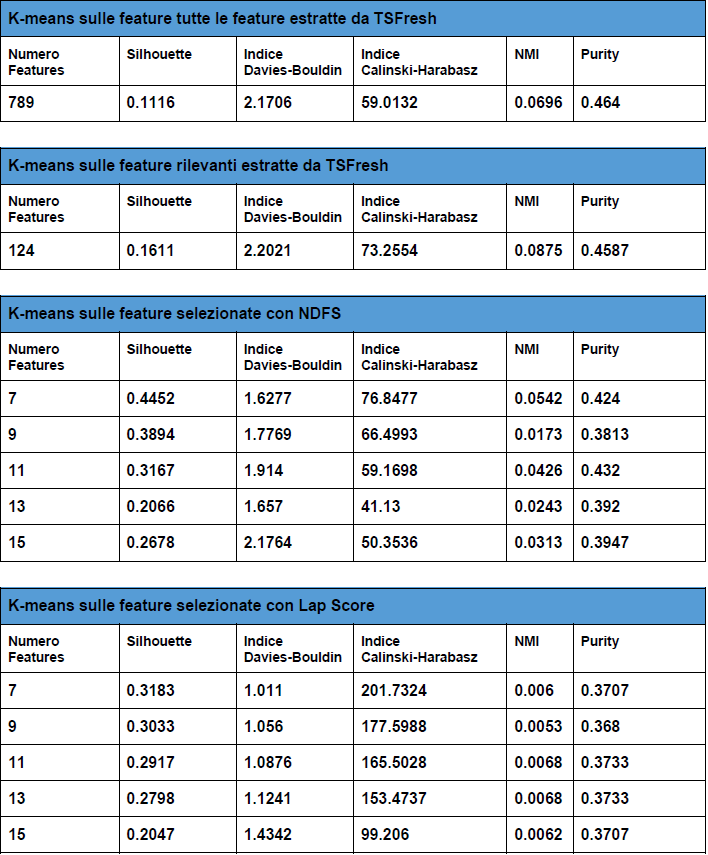
\includegraphics[width=0.9\linewidth]{av/refrigeration_av.png}
	\caption{RefrigerationDevices con tecniche di feature extraction and selection.\\
	\\
	\textbf{L'autoencoder ha purity simile a tutti e quattro gli algoritmi, a meno di leggere differenza}, mentre ha silhouette e DB ben peggiori rispetto a tutti gli algoritmi. In particolare, la silhouette migliora con NDFS e Lap Score.}
	\label{fig:refrigeration_av}
\end{figure}

\subsubsection{TwoLeadECG}
\begin{figure}[H]
	\centering
	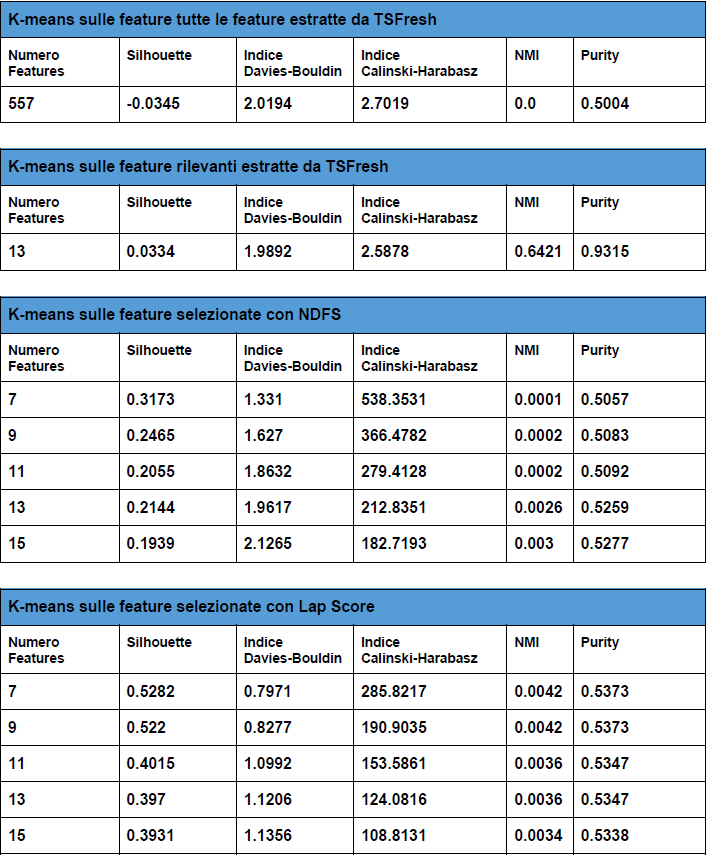
\includegraphics[width=0.9\linewidth]{av/twoleadecg_av.png}
	\caption{TwoLeadECG con tecniche di feature extraction and selection.\\
	\\
	\textbf{L'autoencoder ha silhouette e DB mediamente migliori di tutti e quattro gli algoritmi}, infatti ci sono alcune esecuzioni di Lap Score dove invece si ha una situazione ribaltata. La purity è simile in quasi tutti i casi.}
	\label{fig:twoleadecg_av}
\end{figure}

\subsubsection{TwoPatterns}
\begin{figure}[H]
	\centering
	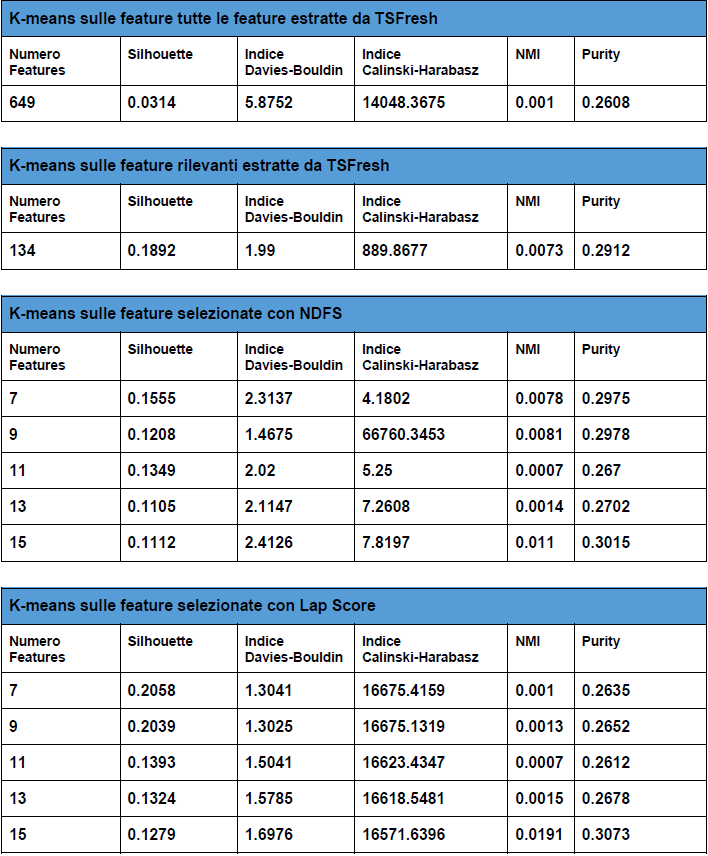
\includegraphics[width=0.9\linewidth]{av/twopatterns_av.png}
	\caption{TwoPatterns con tecniche di feature extraction and selection.\\
	\\
	\textbf{L'autoencoder ha silhouette e DB di gran lunga peggiori rispetto ai quattro algoritmi}, tuttavia la silhouette dei quattro algoritmi è comunque molto bassa. La purity è molto simile in tutti casi, sebbene anche essa risulti molto bassa.}
	\label{fig:twopatterns_av}
\end{figure}